\documentclass[11pt]{article}
\usepackage{graphicx}
\usepackage{hyperref}
\usepackage{geometry}
\geometry{margin=1in}

\title{Predicting Auto Insurance Claim Likelihood using Ensemble Learning under Extreme Class Imbalance}
\author{Sukaina D. Alkhalidy \\ Michigan State University \\ \texttt{alkhali5@msu.edu}}
\date{October 2025 \\ \url{https://github.com/sukaina13/cmse492_project}}

\begin{document}
\maketitle

\section*{Abstract}
This project investigates predicting whether an auto insurance policyholder will file a claim within the next year using the Porto Seguro Safe Driver dataset. The dataset is highly imbalanced, with only about 3.6\% of cases corresponding to claims. To handle this imbalance, ensemble learning methods such as the Balanced Random Forest and EasyEnsembleClassifier are applied and compared to simpler baselines like a majority-class model and logistic regression. Preliminary results show that the EasyEnsemble model improves recall for the minority class from 0.00 to approximately 0.58 and achieves an AUC of 0.63, indicating that ensemble-based resampling can significantly enhance risk prediction performance. The project aims to develop interpretable models that help insurers assess risk more fairly and efficiently.

\section{Background and Motivation}
Insurance providers face significant financial risk due to uncertainty in claim prediction. Accurately modeling the probability of a policyholder filing a claim enables better premium pricing and resource allocation. Traditional models such as logistic regression are limited by their sensitivity to class imbalance, leading to poor recall for rare claim events. Ensemble learning methods, especially balanced bagging and boosting approaches, offer robustness by resampling the minority data and aggregating decision trees. This project explores these methods to improve predictive reliability and interpretability for insurance claim prediction.

\section{Data Description}
The dataset originates from Porto Seguro, a Brazilian insurance company, and was released through a Kaggle competition. It includes 595,212 training samples and 58 predictive features capturing driver demographics, vehicle characteristics, and regional attributes. About 3.6\% of policyholders filed claims, resulting in an extreme class imbalance ratio of roughly 26:1. Missing data primarily occurs in a few categorical variables, while most features are complete and numeric.
\begin{figure}[h]
    \centering
    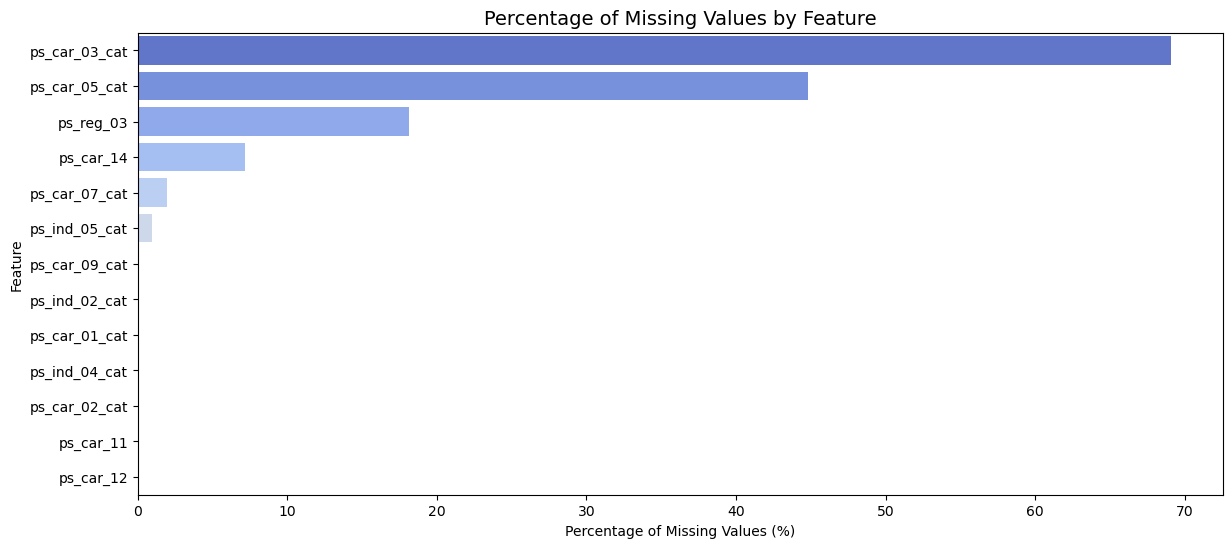
\includegraphics[width=0.8\textwidth]{../figures/missing_barplot.png}
    \caption{Percentage of missing values across major features.}
\end{figure}

\begin{figure}[h]
    \centering
    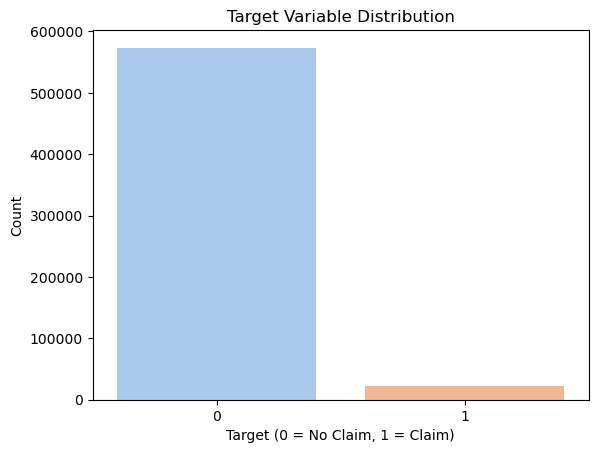
\includegraphics[width=0.8\textwidth]{../figures/target_distribution.png}
    \caption{Target variable distribution showing 96.4\% no-claim and 3.6\% claim cases.}
\end{figure}

Planned preprocessing includes imputing missing values with median/mode, dropping columns with over 50\% missingness, and using label encoding for categorical variables. Since tree-based methods are insensitive to scaling, normalization is not required.

\section{Proposed Methodology}
Three models of increasing complexity are compared:
\begin{enumerate}
    \item \textbf{Majority Class Baseline:} Always predicts no claim.
    \item \textbf{Logistic Regression:} Incorporates class weighting to account for imbalance.
    \item \textbf{Ensemble Models:} Balanced Random Forest and EasyEnsembleClassifier, both of which combine resampling with tree-based learners.
\end{enumerate}
\begin{figure}[h]
    \centering
    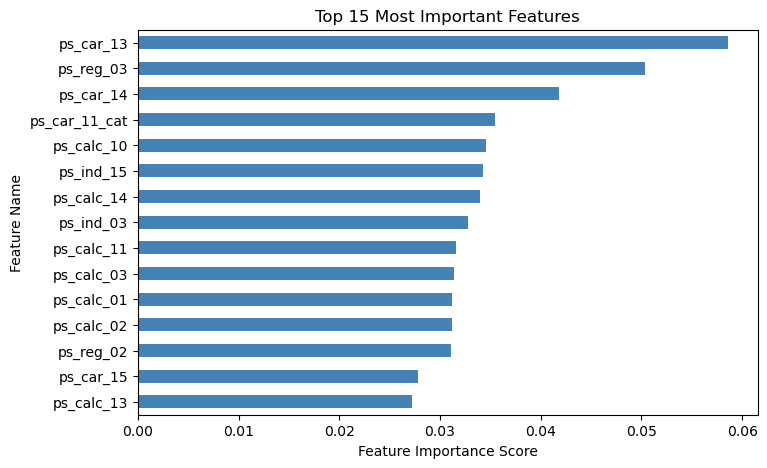
\includegraphics[width=0.8\textwidth]{../figures/feature_importance_balanced_rf.png}
    \caption{Top 15 most important features identified by Balanced Random Forest.}
\end{figure}
Model interpretability is enhanced through feature importance plots, while hyperparameter tuning via RandomizedSearchCV ensures optimal performance. EasyEnsemble is expected to outperform due to its adaptive boosting strategy over balanced subsets.

\section{Evaluation Framework}
Performance will be evaluated using precision, recall, F1-score, and area under the ROC curve (AUC). A stratified 70/15/15 train-validation-test split preserves class ratios. The baseline majority model serves as a reference point with 96.4\% accuracy but zero recall. Success will be defined as achieving recall above 0.55 and AUC above 0.65 for the minority class, improving both detection and ranking ability for true claim cases.

\section{Timeline and Milestones}
\begin{itemize}
    \item \textbf{Week 9 (Oct 28–Nov 3):} Complete exploratory data analysis and baseline models.
    \item \textbf{Week 10–11:} Implement ensemble models and conduct hyperparameter tuning.
    \item \textbf{Week 12:} Evaluate results and refine interpretability analysis.
    \item \textbf{Week 13–14:} Draft final report and prepare presentation.
    \item \textbf{Week 15 (Dec 2–8):} Final presentation and submission.
\end{itemize}

\begin{figure}[h]
    \centering
    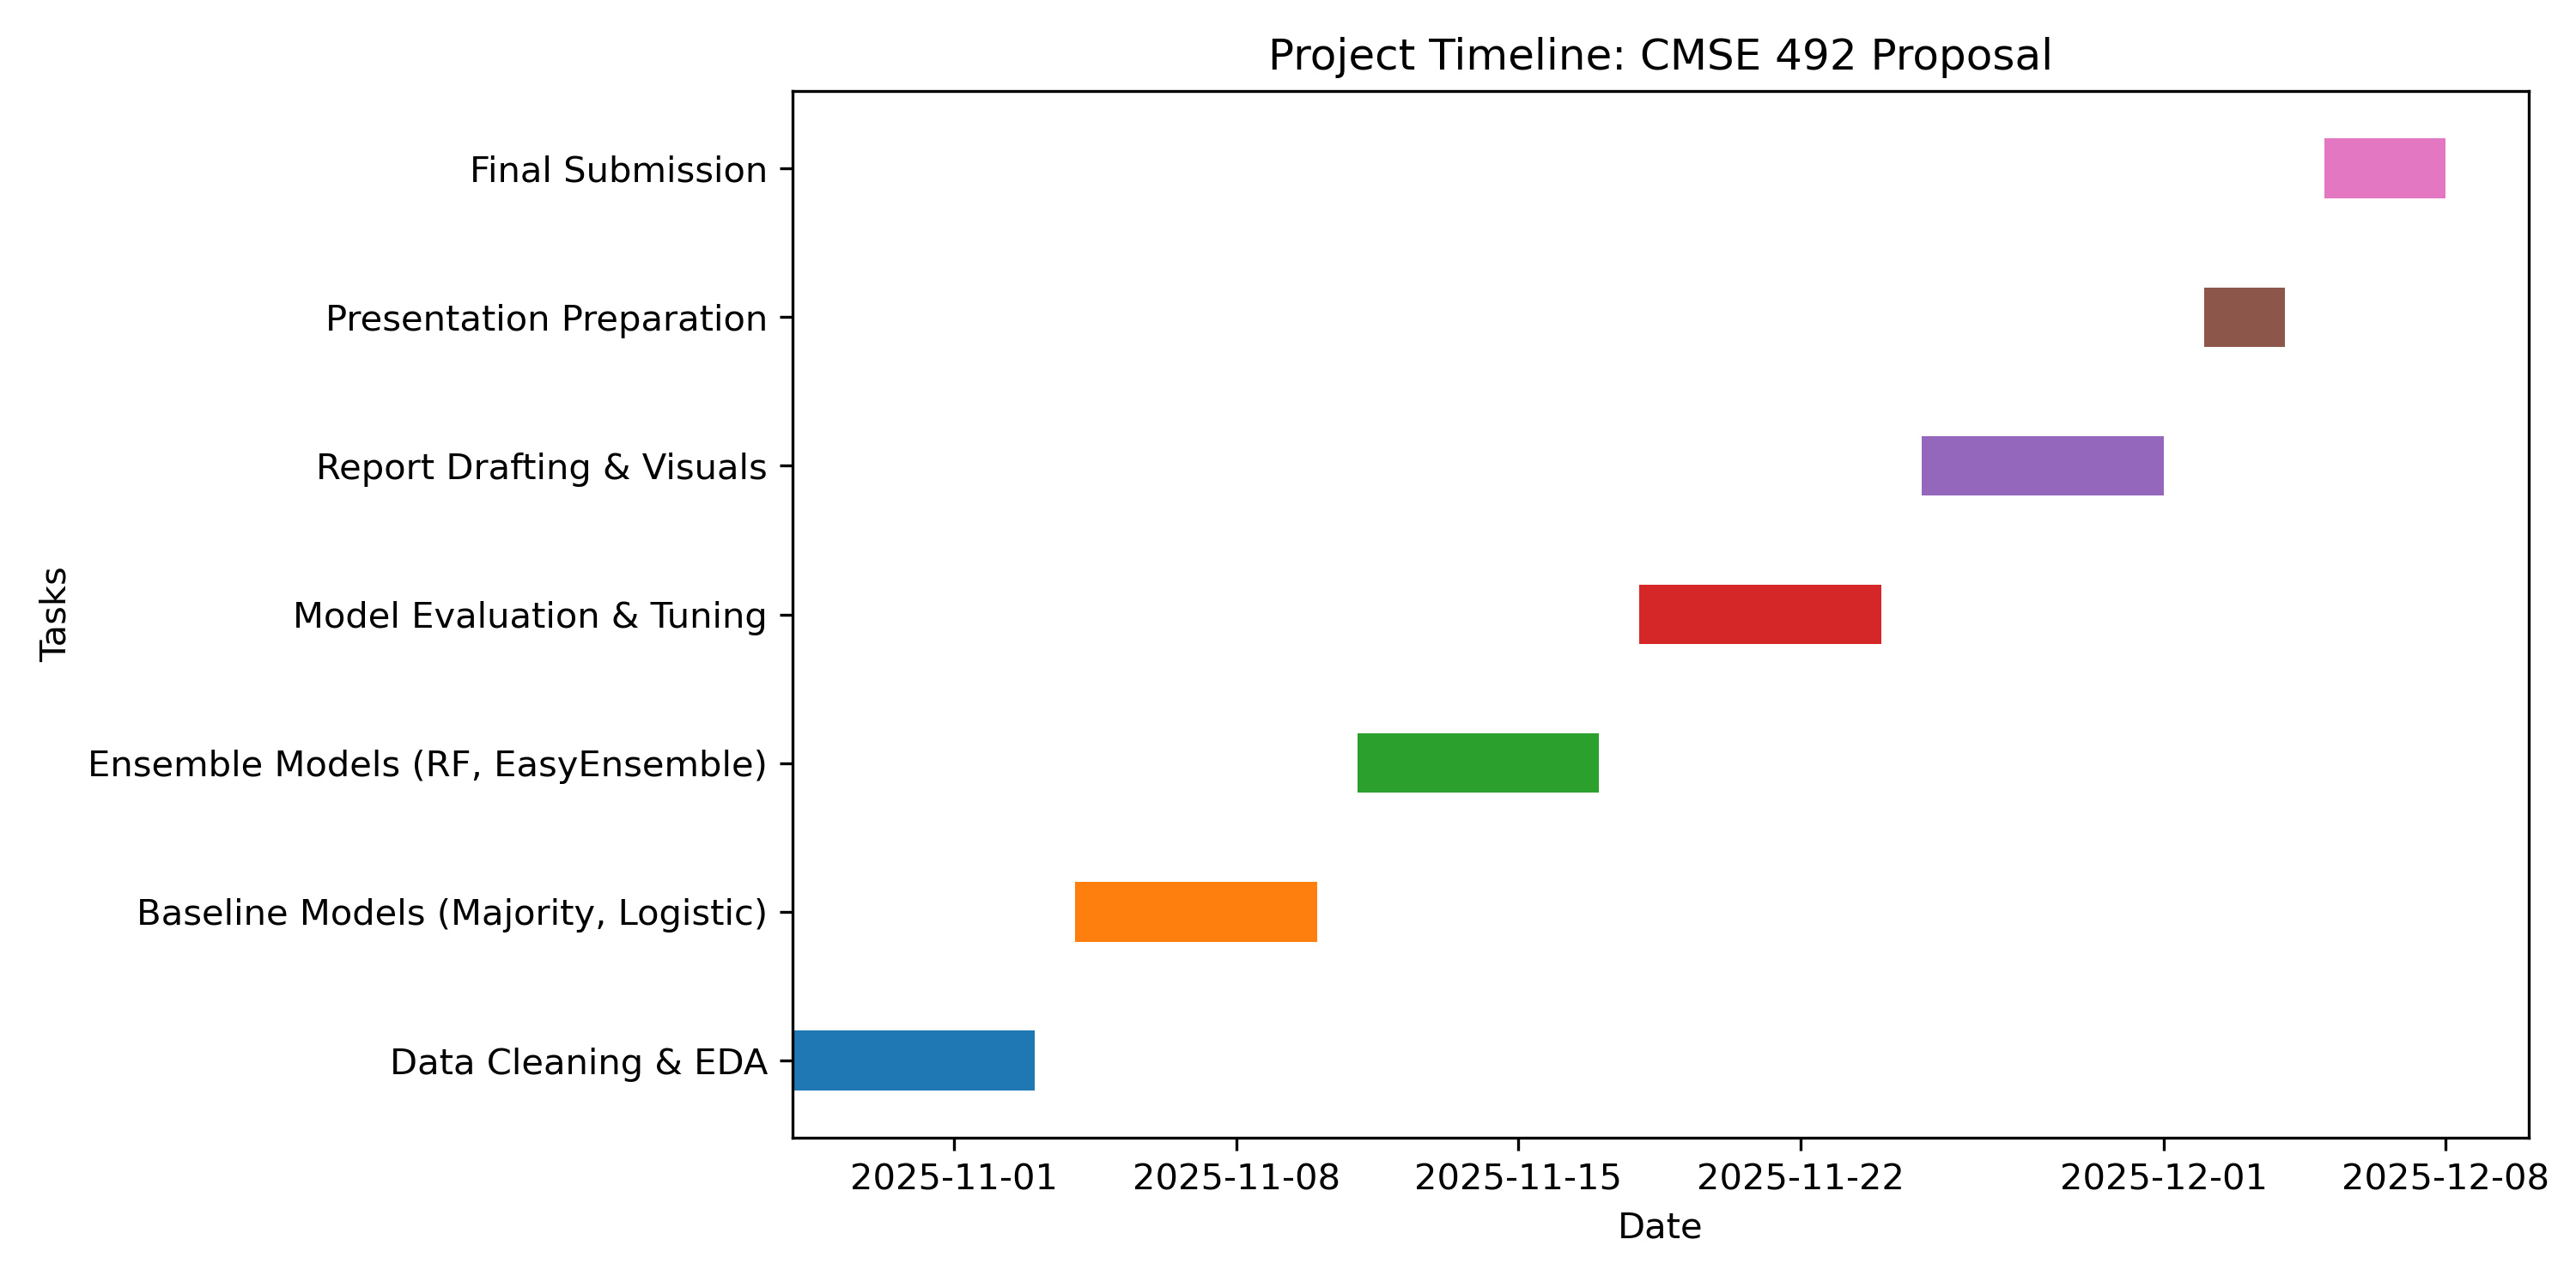
\includegraphics[width=0.9\textwidth]{../figures/gantt_chart.png}
    \caption{Planned Gantt chart outlining project tasks and milestones.}
\end{figure}

\end{document}
\documentclass[11pt]{article}
\usepackage{graphicx}
\usepackage{geometry}
\usepackage{hyperref}
\usepackage{setspace}
\geometry{margin=1in}
\setstretch{1.15}

\title{\textbf{Predicting Auto Insurance Claim Likelihood Using Ensemble Learning Under Extreme Class Imbalance}}
\author{
Sukaina D. Alkhalidy \\
\texttt{alkhal13@msu.edu} \\
October 2025 \\
\href{https://github.com/sukaina13/cmse492_project}{https://github.com/sukaina13/cmse492\_project}
}
\date{}

\begin{document}
\maketitle

\section*{Abstract}
Predicting whether an auto insurance policyholder will file a claim in the next year is an important problem for both financial planning and fair risk assessment. This project explores how machine learning can improve claim prediction using the Porto Seguro Safe Driver dataset, a large and highly imbalanced dataset where only about 3.6\% of policyholders made a claim. I compare simple baseline models such as predicting the majority class and logistic regression with more advanced ensemble methods like Balanced Random Forest and EasyEnsemble, which are designed to handle class imbalance effectively.

Preliminary results show that the EasyEnsemble model performs much better at identifying claim cases, increasing recall from 0.00 to around 0.58 and achieving an area under the ROC curve (AUC) of 0.63. These findings suggest that ensemble-based approaches can improve fairness and accuracy in predicting rare insurance claims. Ultimately, this project aims to build interpretable, data-driven models that help insurance companies make more informed and equitable decisions when assessing driver risk.

\section{Background and Motivation}
Predicting whether a driver will file an insurance claim is one of the most important and challenging tasks in the insurance industry. Each year, companies must decide how to set fair premiums while maintaining profitability and protecting customers from unfair pricing. A model that can accurately estimate the likelihood of a claim allows insurers to manage financial risk, detect potential fraud, and better allocate resources for claims investigation. However, the key challenge lies in the data itself—claim events are extremely rare, occurring in only about 3–4\% of all cases, which makes accurate prediction very difficult.

Traditional statistical methods, such as logistic regression and generalized linear models, have long been used in insurance analytics. While these approaches are simple and interpretable, they tend to struggle with highly imbalanced datasets. In these cases, they often predict the majority class (“no claim”) almost exclusively, achieving high overall accuracy but poor recall for the minority class—the actual claim cases that matter most. This imbalance leads to models that appear strong on paper but fail in practice, where missing a true claim can lead to major financial losses.

Machine learning offers a better way to handle this challenge. Ensemble-based models such as Balanced Random Forest and EasyEnsemble are designed to correct class imbalance by training on balanced subsets of data and combining their predictions. These models can identify rare claim cases more effectively while still maintaining generalization. They also produce interpretable results, such as feature importance rankings, which can reveal which policyholder or vehicle characteristics are most predictive of risk.

The goal of this project is to develop and evaluate such ensemble learning models to improve the accuracy and fairness of claim prediction. By comparing baseline models (like logistic regression and majority-class prediction) with advanced ensemble methods, this project aims to demonstrate how data-driven approaches can enhance risk modeling and provide actionable insights for insurance companies.

\section{Data Description}
The dataset used in this project originates from Porto Seguro, one of Brazil’s largest auto and home insurance companies. It was released as part of the 2017 Kaggle competition \textit{“Porto Seguro’s Safe Driver Prediction,”} organized by Addison Howard, Adriano Moala, and Walter Reade. The dataset was collected internally by Porto Seguro through customer records, vehicle data, and claim history, and was shared to encourage innovation in risk modeling. The goal was to improve claim prediction accuracy so insurers could offer fairer pricing—lower premiums for safe drivers and more accurate risk assessment for higher-risk individuals.

The training dataset contains 595,212 records and 59 variables, including 58 predictive features and one binary target variable. The features include demographic data (\texttt{ps\_ind\_*}), vehicle characteristics (\texttt{ps\_car\_*}), regional indicators (\texttt{ps\_reg\_*}), and engineered risk scores (\texttt{ps\_calc\_*}).

From exploratory analysis, the dataset shows a severe class imbalance: only 3.6\% of policyholders filed claims. Some features such as \texttt{ps\_car\_03\_cat} and \texttt{ps\_car\_05\_cat} have large amounts of missing data (69\% and 45\%, respectively), while the rest are mostly complete.

Preprocessing steps include imputing missing values with median (numerical) or mode (categorical), dropping features with more than 50\% missingness, and label encoding categorical variables. Since tree-based models are scale-invariant, feature scaling is not required. These steps ensure the data is clean, consistent, and ready for robust training.

Two figures summarize the dataset:
\begin{itemize}
    \item \textbf{Figure 1:} Missing value rates by feature.
    \item \textbf{Figure 2:} Target class imbalance.
\end{itemize}

\section{Proposed Methodology}
This is a supervised learning problem framed as binary classification: predicting whether a driver will file an insurance claim in the next year. The goal is to identify the minority “claim” class accurately while avoiding bias toward the majority “no claim” class.

To compare performance across complexity levels, three models will be tested:
\begin{enumerate}
    \item \textbf{Majority Class Baseline} – Always predicts “no claim.” Serves as a benchmark for imbalance problems.
    \item \textbf{Weighted Logistic Regression} – A linear, interpretable model with class weighting to compensate for imbalance.
    \item \textbf{Ensemble Models (Balanced Random Forest, EasyEnsembleClassifier)} – Advanced tree-based methods that rebalance and boost data to capture nonlinear relationships and improve recall.
\end{enumerate}

Model complexity increases from simple to advanced:  
Baseline (no learning), Logistic Regression (low complexity), and Ensemble Models (high complexity capturing feature interactions).

The workflow follows these steps:
\begin{enumerate}
    \item Clean and preprocess the dataset.
    \item Perform stratified train/validation/test split.
    \item Train and tune models with cross-validation.
    \item Evaluate using accuracy, recall, precision, F1, and ROC–AUC.
    \item Visualize results with ROC curves, confusion matrices, and feature importance plots.
\end{enumerate}

\section{Evaluation Framework}
Because the dataset is highly imbalanced, accuracy alone isn’t enough. A model that always predicts “no claim” would achieve high accuracy but fail to identify true positives.

The metrics used include:
\begin{itemize}
    \item \textbf{Recall} – measures how many true claim cases are caught.
    \item \textbf{Precision} – measures how many predicted claims are actually correct.
    \item \textbf{F1-score} – balances recall and precision.
    \item \textbf{AUC (ROC)} – evaluates model separability across thresholds.
\end{itemize}

A stratified 70/15/15 train-validation-test split ensures both classes are represented equally.  
The baseline model sets the floor: high accuracy but recall = 0. Advanced models will be evaluated against it.

The project will be considered successful if:
\begin{itemize}
    \item Recall $\geq$ 0.55
    \item AUC $\geq$ 0.65
    \item Noticeably higher F1-score than the baseline
\end{itemize}

\section{Timeline and Milestones}
This project runs from late October through December 8, 2025.
\begin{itemize}
    \item Week 1: Data cleaning and EDA
    \item Weeks 2–3: Build baseline and logistic regression models
    \item Weeks 4–5: Train ensemble models (Balanced RF, EasyEnsemble)
    \item Week 6: Evaluate and tune models
    \item Week 7: Write report and create figures
    \item Week 8 (Dec 2–4): Prepare presentation
    \item Week 9 (Dec 5–8): Final submission
\end{itemize}

A Gantt chart (Figure 3) visualizes the full timeline and dependencies between tasks.  
Critical milestones include model evaluation and final reporting, with buffer time for debugging or retraining. The schedule aligns with course deadlines and allows flexibility for unforeseen issues.

\begin{figure}[h]
    \centering
    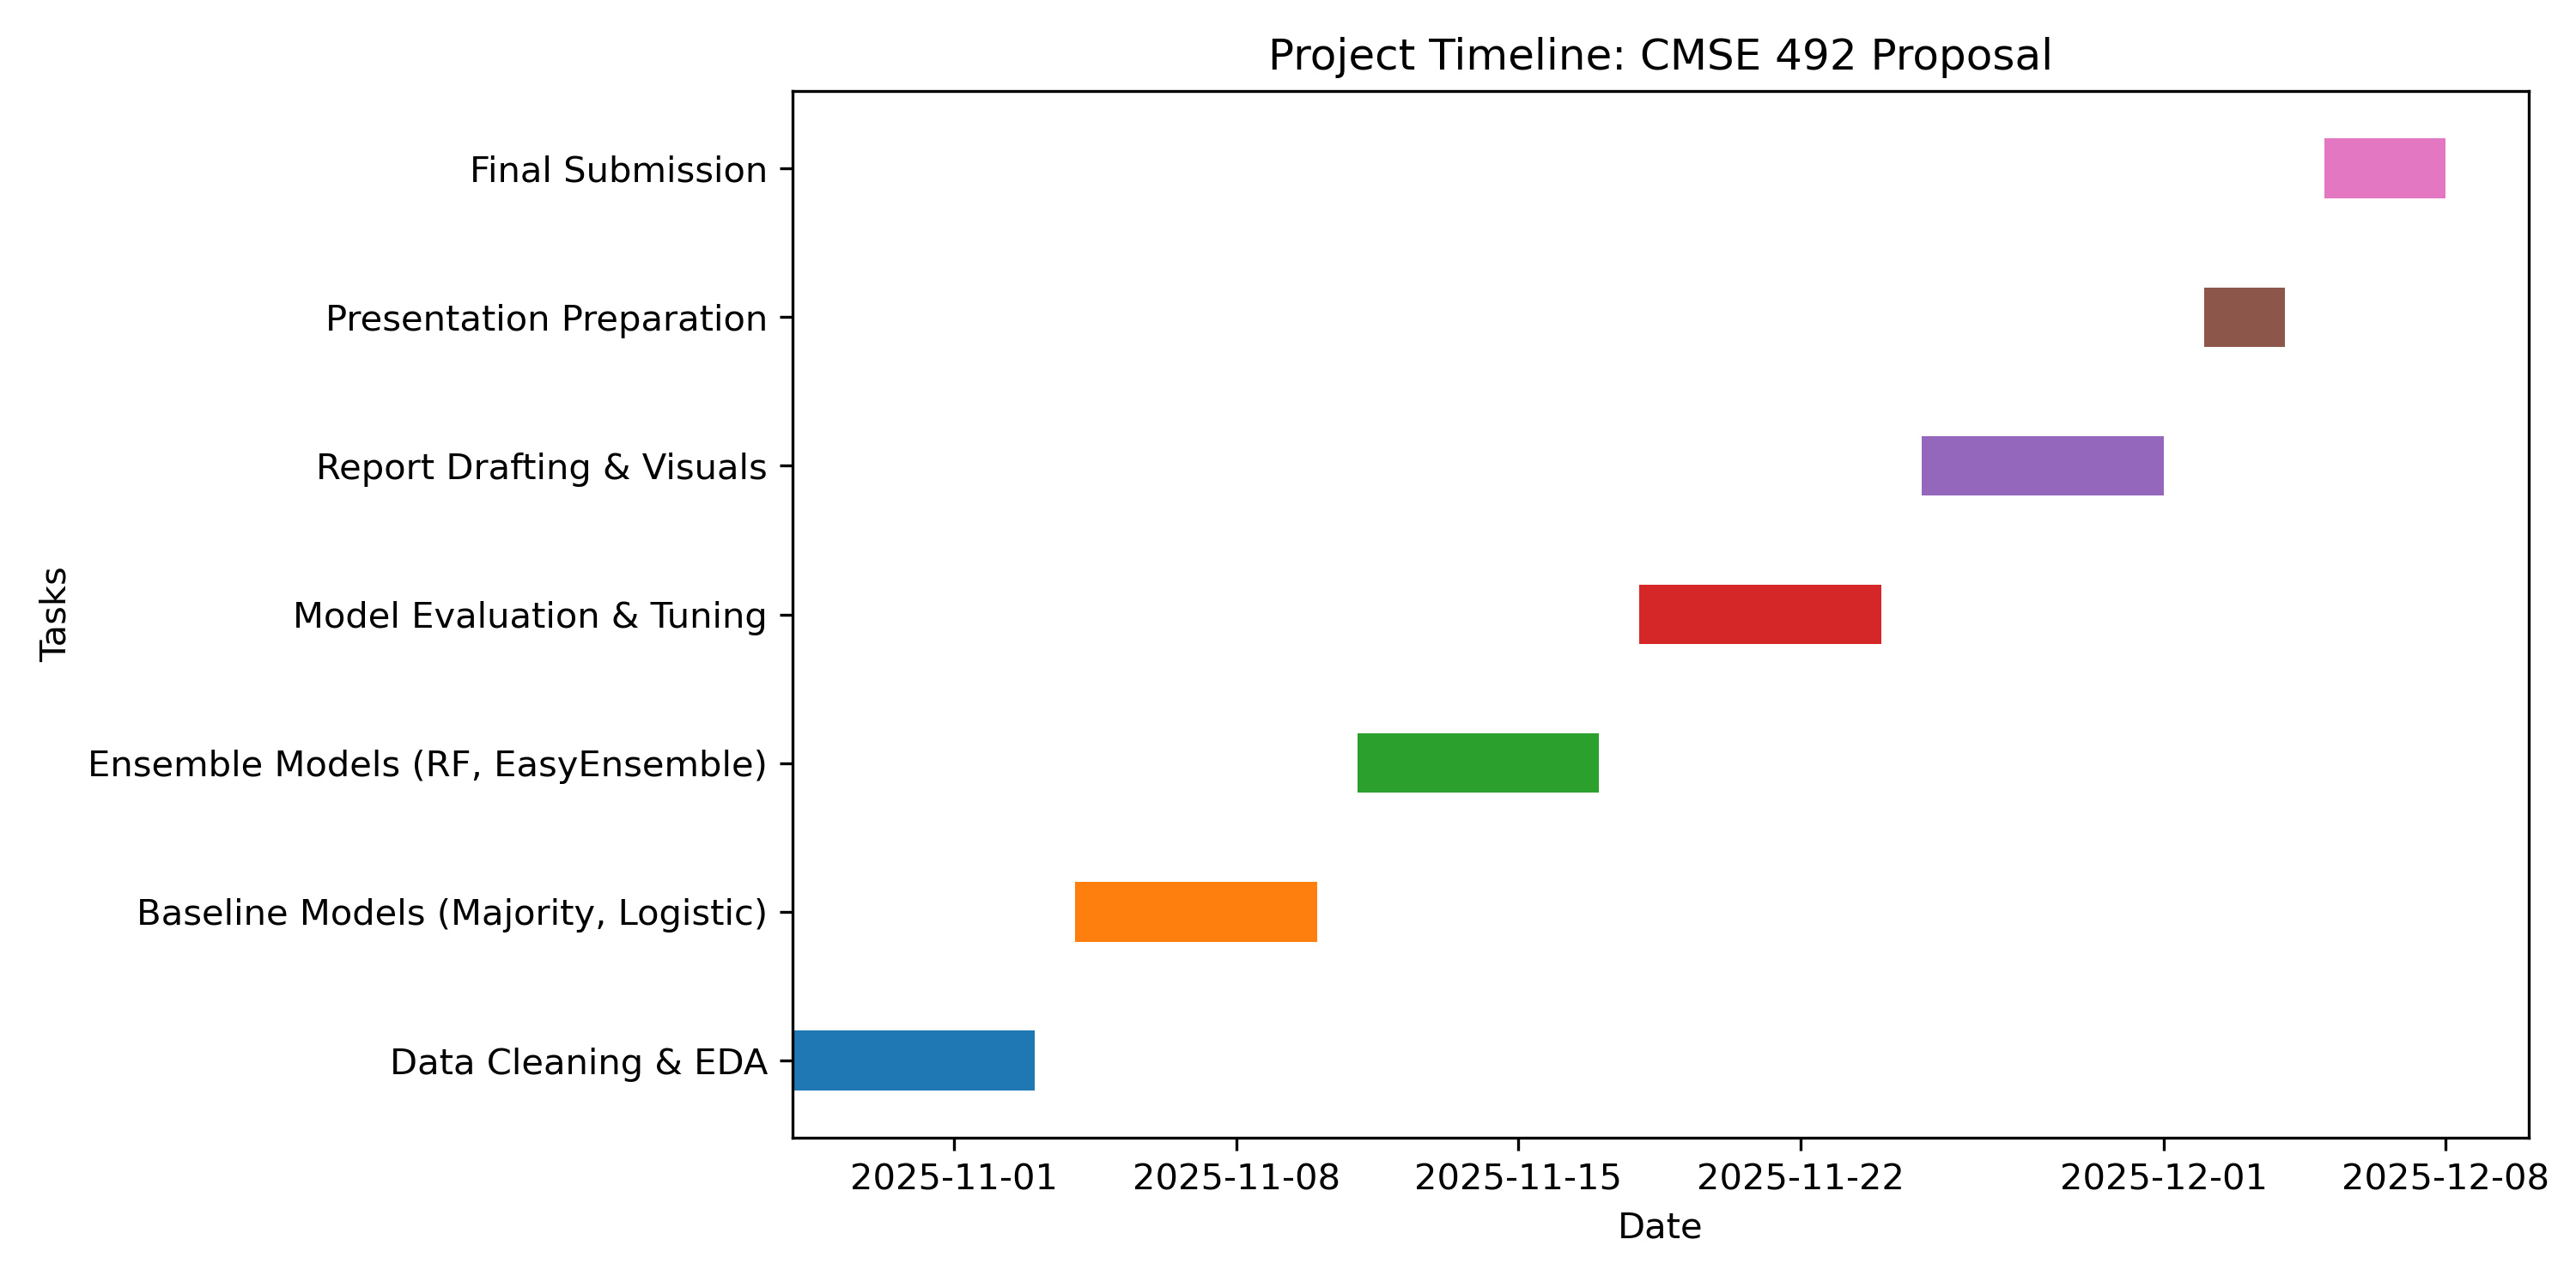
\includegraphics[width=0.9\textwidth]{../figures/gantt_chart.png}
    \caption{Project timeline and milestones for CMSE 492.}
\end{figure}

\end{document}
